\documentclass[12pt,a4paper]{article}
%\usepackage[allfiguresdraft]{draftfigure}
%\newcommand{\pdfextension}{pdf}
%\newcommand{\pngextension}{png}
\usepackage{cite}
\usepackage{natbib}
\usepackage{breakcites}
\usepackage[normalem]{ulem}
\usepackage{comment}
\usepackage[font=footnotesize,labelfont=bf]{caption}
 \usepackage[dvipsnames]{xcolor}
\let\rho=\varrho

\def\fref#1{Fig.~\ref{#1}}
\def\tabref#1{Table~\ref{#1}}
\def\cref#1{Condition~\ref{#1}}
\def\Cref#1{Corollary~\ref{#1}}
\def\eref#1{(\ref{#1})}
\def\sref#1{\textsection\ref{#1}}
\def\lref#1{Lemma~\ref{#1}}
\def\rref#1{Remark~\ref{#1}}
\def\tref#1{Theorem~\ref{#1}}
\def\dref#1{Definition~\ref{#1}}
\def\pref#1{Proposition~\ref{#1}}
\def\aref#1{Assumption~\ref{#1}}
\def\qref#1{Subsection~\ref{#1}}

\def\dref#1{Definition~\ref{#1}}
\def\myundefined#1{\special{ps: 1 0 0 setrgbcolor}{what is #1?}%
	\special{ps: 0 0 0 setrgbcolor}}
\newenvironment{myitem}
{\begin{itemize}
  \setlength{\itemsep}{1pt}
  \setlength{\parskip}{0pt}
  \setlength{\parsep}{0pt}}
{\end{itemize}}

\newenvironment{myenum}
{\begin{enumerate}
  \setlength{\itemsep}{1pt}
  \setlength{\parskip}{0pt}
  \setlength{\parsep}{0pt}}
{\end{enumerate}}

%\usepackage{sub_JP}
%\usepackage{fancyhdr}
%\pagestyle{fancy}
\usepackage{amsmath}
\usepackage{amsfonts}
\usepackage{graphicx}
%\usepackage{makeidx}
\usepackage{times}
\usepackage{amsthm}
\usepackage{ amssymb }
\usepackage{color}
\usepackage{mhequ}
\usepackage{dsfont}
\usepackage[scanall]{psfrag}
\usepackage[margin=2.5cm]{geometry}
\usepackage{color}
\usepackage{url}
\usepackage{lipsum}
%\usepackage{authblk}
\usepackage{subfig}
\usepackage{mhequ}

\usepackage{tikz}
\usepackage[graphics, active, tightpage]{}

%\usepackage[expansion=true]{microtype}

%\captionsetup[figure]{margin=2cm,font=footnotesize,labelfont=bf,labelsep=endash,textfont=rm}\captionsetup[subfigure]{margin=0pt}


\def\thecomma{\ifx,\thenewxt \else\ifx;\thenext \else\ifx.\thenext
	\else\ifx!\thenext \else\ifx:\thenext\else\ifx)\thenext \else \
	\fi\fi\fi\fi\fi\fi}
\def\condblank{\futurelet\thenext\thecomma}
\def\ie{{\it i.e.,}\condblank}
\def\eg{{\it e.g.,}\condblank}

\numberwithin{equation}{section}



\newtheorem*{oneshot}{Hypothesis~\ref{h:assumption}}
\newtheorem{theorem}{Theorem}[section]
\newtheorem{lemma}[theorem]{Lemma}
\newtheorem{proposition}[theorem]{Proposition}
\newtheorem{definition}[theorem]{Definition}
\newtheorem{notation}[theorem]{Notation}
\newtheorem{observation}[theorem]{Observation}
\newtheorem{assumption}[theorem]{Assumption}
\newtheorem{hypothesis}[theorem]{Hypothesis}
\newtheorem{conjecture}[theorem]{Conjecture}
\newtheorem{example}[theorem]{Example}
\newtheorem{property}[theorem]{Property}
\newtheorem{condition}[theorem]{Condition}
\newtheorem{corollary}[theorem]{Corollary}
\theoremstyle{definition} %remarks in rm
\newtheorem{remark}[theorem]{Remark}
\def\HALF{{\textstyle\frac{1}{2}}}
\def\TWOTHIRDS{{\textstyle\frac{2}{3}}}
\def\FOURTHIRDS{{\textstyle\frac{4}{3}}}
%\bibliographystyle{JPE}
%\usepackage{cite}

\usepackage{stmaryrd}
\def\scomm#1#2{\ensuremath{\bigr\llbracket #1:#2\bigr\rrbracket}}

\newcommand{\meq}[1]{\ensuremath{\stackrel{\scriptscriptstyle#1}{\scriptstyle
			\sim}}}


\newcommand{\dd}{\mathrm{d}}
\newcommand{\dt}{\,\dd t}
\newcommand{\mpart}[2]{\frac{\partial #1}{\partial #2}}
\newcommand{\avg}[1]{\left\langle #1\right\rangle}

\newcommand{\bigoh}[1]{\hat {\mathcal O}(p_2^{#1})}
\newcommand{\bigohneg}[1]{\hat {\mathcal O}\!\left({p_2^{-#1}}\right)}

\newcommand{\jp }[1]{{\color{magenta}jp*****:  #1}}
\newcommand{\noe }[1]{{\color{red}noe:  #1}}
\newcommand{\christophe }[1]{{\color{red}christophe: #1}}
\def\argcdot{{\,\cdot\,}}


\newcommand{\cA}{{\ensuremath{\mathcal A}} }
\newcommand{\cF}{{\ensuremath{\mathcal F}} }
\newcommand{\cP}{{\ensuremath{\mathcal P}} }
\newcommand{\cE}{{\ensuremath{\mathcal E}} }
\newcommand{\cH}{{\ensuremath{\mathcal H}} }
\newcommand{\cC}{{\ensuremath{\mathcal C}} }
\newcommand{\cN}{{\ensuremath{\mathcal N}} }
\newcommand{\cL}{{\ensuremath{\mathcal L}} }
\newcommand{\cT}{{\ensuremath{\mathcal T}} }
\newcommand{\cD}{{\ensuremath{\mathcal D}} }
\newcommand{\cU}{{\ensuremath{\mathcal U}} }
\newcommand{\cV}{{\ensuremath{\mathcal V}} }
\newcommand{\cS}{{\ensuremath{\mathcal S}} }
\newcommand{\cY}{{\ensuremath{\mathcal Y}} }


%%%%%%%%%%%%%%%%%%%%%%%%%%%%%%%%%%%%%%%%%%%%%%%%%%%%%%%%%%%%%%%%%%%%%%%%%%%%%%
%%%%%%%%%%%% Blackboard bolds
%%%%%%%%%%%%%%%%%%%%%%%%%%%%%%%%%%%%%%%%%%%%%%%%%%%%%%%%%%%%%%%%%%%%%%%%%%%%%%

\newcommand{\bbA}{{\ensuremath{\mathbb A}} }
\newcommand{\bbB}{{\ensuremath{\mathbb B}} }
\newcommand{\bbC}{{\ensuremath{\mathbb C}} }
\newcommand{\bbD}{{\ensuremath{\mathbb D}} }
\newcommand{\bbE}{{\ensuremath{\mathbb E}} }
\newcommand{\bbF}{{\ensuremath{\mathbb F}} }
\newcommand{\bbG}{{\ensuremath{\mathbb G}} }
\newcommand{\bbH}{{\ensuremath{\mathbb H}} }
\newcommand{\bbI}{{\ensuremath{\mathbb I}} }
\newcommand{\bbJ}{{\ensuremath{\mathbb J}} }
\newcommand{\bbK}{{\ensuremath{\mathbb K}} }
\newcommand{\bbL}{{\ensuremath{\mathbb L}} }
\newcommand{\bbM}{{\ensuremath{\mathbb M}} }
\newcommand{\bbN}{{\ensuremath{\mathbb N}} }
\newcommand{\bbO}{{\ensuremath{\mathbb O}} }
\newcommand{\bbP}{{\ensuremath{\mathbb P}} }
\newcommand{\bbQ}{{\ensuremath{\mathbb Q}} }
\newcommand{\bbR}{{\ensuremath{\mathbb R}} }
\newcommand{\bbS}{{\ensuremath{\mathbb S}} }
\newcommand{\bbT}{{\ensuremath{\mathbb T}} }
\newcommand{\bbU}{{\ensuremath{\mathbb U}} }
\newcommand{\bbV}{{\ensuremath{\mathbb V}} }
\newcommand{\bbW}{{\ensuremath{\mathbb W}} }
\newcommand{\bbX}{{\ensuremath{\mathbb X}} }
\newcommand{\bbY}{{\ensuremath{\mathbb Y}} }
\newcommand{\bbZ}{{\ensuremath{\mathbb Z}} }


%%%%%%%%%%%%%%%%%%%%%%%%%%%%%%%%%%%%%%%%%%%%%%%%%%%%%%%%%%%%%%%%%%%%%%%%%%%%%%
%%%%%%%%%%%% Greek letters
%%%%%%%%%%%%%%%%%%%%%%%%%%%%%%%%%%%%%%%%%%%%%%%%%%%%%%%%%%%%%%%%%%%%%%%%%%%%%%

\newcommand{\ga}{\alpha}
\newcommand{\gb}{\beta}
\newcommand{\gga}{\gamma}            % \gg already exists...
\newcommand{\gd}{\delta}
\newcommand{\gep}{\varepsilon}       % \ge already exists...
\newcommand{\gp}{\varphi}
\newcommand{\gr}{\rho}
\newcommand{\gvr}{\varrho}
\newcommand{\gz}{\zeta}
\newcommand{\gG}{\Gamma}
\newcommand{\gP}{\Phi}
\newcommand{\gD}{\Delta}
\newcommand{\gk}{\kappa}
\newcommand{\go}{\omega}
\newcommand{\gto}{{\tilde\omega}}
\newcommand{\gO}{\Omega}
\newcommand{\gl}{\lambda}
\newcommand{\gL}{\Lambda}
\newcommand{\gs}{\sigma}
\newcommand{\gS}{\Sigma}
\newcommand{\gt}{\vartheta}
\let\kappa=\varkappa
\let\phi=\varphi
\def\CC{{\mathcal C}}
\def\Rsch{r_{\rm sch}}
\def\d{{\rm d}} 
\def\KK{{\mathcal K}}
\def\OO{{\mathcal O}}
\def\integer{{\mathbb Z}}
\def\real{{\mathbb R}}
\newcommand{\ind}{\mathbf{1}}
\def\p2t2{{\tilde p_2^{\,2}}}

\def\fhc#1{\textcolor{violet}{#1}}
\definecolor{bittersweet}{rgb}{1.0, 0.44, 0.37}
\newcommand{\fhn}[1]{{\textcolor{bittersweet}{\sf[#1]}}}
\newcommand{\edit}[2] {\textcolor{black}{\sout{#1}} {\textcolor{violet}{#2}} }
\newcommand{\HZ}[1]{\textcolor{ForestGreen}{HZ:#1}}
\def\JP#1{\textcolor{blue}{JPE:#1}}
\let\epsilon=\varepsilon
\usepackage{authblk}

%%%%%%%
%% Farbod Hassani
%%%%%%%
\newcommand{\HH}{\mathcal H}
\def\be{\begin{equation}}
\def\ee{\end{equation}}
\def\const{\text{const.}}
\def\citep#1{[#1]}
\begin{document}
\section{Context}
The effective field theories (EFT) are considered in physics to approximate a fundamental theory (e.g., appearing in cosmology, quantum field theory, statistical mechanics and etc \citep{Pich:1998xt, HARTMANN2001267,Cheung:2007st, Gubitosi:2012hu,Weinberg:2008hq  }),  with an appropriate degrees of freedom. The EFT is valid up to a certain energy scale/length scale, while the extra degrees of  freedom belonging to high energy/small scales can be integrated out. The EFT of dark energy, $k$-essence specifically, has been a popular tool for cosmologists to consider the late-time accelerated expansion of the Universe \citep{SupernovaSearchTeam:1998fmf}. The scalar field ($\Pi$) equation, relevant for cosmological studies in this framework \citep{Hassani:2019lmy,Hassani:2019wed} obeys a second order non-linear partial differential equation (PDE). Among all terms, the relevant PDE based on the numerical studies using $k$-evolution $N$-body code \code{Hassani:2019lmy} reads,
\begin{equ}
  \partial_t^2 \Pi=\alpha (\nabla_x\Pi)^2 +\beta \Delta \Pi~.
\end{equ}
The initial conditions for this equation are given by a source field
$\Phi$, which is gravitational potential and is generated by density of particles in an $N$-body code\cite{Adamek:2016zes}. We consider then of the form
$\Pi(x,0)=0$,
while $\partial_t\Pi(x,0)$ is some non-zero function.

It was then discovered in \citep{?} that such initial conditions for large $\alpha/\beta$ can
lead to a blowup in finite time,  and that the relation between
$\alpha $ and $\beta $ (called the speed of sound) leads to a subtle
interplay between this divergence, while for $\beta \ne0$ the ``sound
wave'' can lead to another type of divergence.

The aim of this paper is to discuss a 1-dimensional version of this
problem, and to give some proofs and some general remarks about this
phenomenon, which is important in cosmology because xxx.

Admittedly, while this is a modest start, it should be relatively easy
to generalize this to a spherically symmetric situation.

\section{The equations}




We consider the equations
\begin{equ}\label{eq:main}
  u_{tt}-\beta u_{xx}=\alpha (u_x)^2~, \quad \alpha\ne0 ~,
\end{equ}
for $t\ge0$ and $x\in\real$.
When $\beta\ne0$ we define
$u(x,t)=\frac{\beta}{\alpha } v(\sqrt|\alpha| x /\beta  , |\alpha| t
/\beta )$ and obtain
\begin{equ}\label{eq:main1}
  v_{tt}- v_{xx}=(v_x)^2~.
\end{equ}
Thus, it suffices to consider \eref{eq:main1}.\\
When $\beta =0$, we consider the equation
\begin{equ}\label{eq:main2}
  w_{tt}=  (w_x)^2~.
\end{equ}
Equations like (\ref{eq:main})-(\ref{eq:main2}) have been studied in
great detail, but mostly in dimensions 2 and higher. Here, we are
interested in the questions of divergence of such equations (in finite
time). Such questions are of interest in cosmological models. In that
case, it is probably more reasonable to keep \eref{eq:main}, since the
change of variables leading to \eref{eq:main1} will of lead to a
change of the initial conditions. But in cosmology, these initial
conditions are fixed.

The behavior if the solutions can be quite different in the case
$\beta =0$ and $\beta \ne0$. When $\beta =0$, there is no wave
equation and therefore we are confronted with what is essentially a
set of local problems.

In the next section we discuss $\beta =0$ and after that, we discuss
$\beta \ne0$.
\section{The case $\beta =0$}
The following is a slight adaptation of the results of Wittwer, Pan
Shi, and Hassani.


We consider the equation $u_{tt}=(u_x)^2$ on the real line.
We start by writing the solution in the form
\begin{equ}\label{eq:peter}
  u(x,t)=f(x)+g(x)t +\int_0^t \d\tau \int_0^\tau  \d\tau'
  (u_x(x,\tau '))^2~. 
\end{equ}
This corresponds to the initial conditions
\begin{equ}
  u(x,0)=f(x)~,\quad  u_t(x,0)=g(x)~.
\end{equ}
We will consider the case where $f'(0)=g'(0)=0$, and we ask how the
solution behaves near $x=0$. Depending on the curvatures $f''(0)$ and
$g''(0)$, the second derivative $u_{xx}(x,t)$ will, or will not
  diverge at $x=0$. Of course, if the functions $f$ and $g$ have
  vanishing derivatives at some other point(s) $x_0$, the same
  discussion will apply at those points, and there can be one of these
  points where $u_{xx}(x_0,t)$ diverges before the one at $x=0$. In
  the following proposition, we will neglect this aspect.

  
\begin{proposition}\label{prop:peter}
  Assume $f'(0)=g'(0)=0$. Define
  \begin{equ}
    c=\HALF g''(0)^2-\TWOTHIRDS f''(0)^3~. 
  \end{equ}

  Then the following cases appear:\\
  (i) If $g''(0)>0$ then $u_{xx}(0,t)$ diverges in finite time $t_+$
  given by
  \begin{equ}\label{eq:div}
    t_+=\int_{f''(0)}^\infty \frac{\d b }{\sqrt{\FOURTHIRDS b^3 +2c}}~.
  \end{equ}\\
  (ii) If $g''(0)<0$ then $u_{xx}(0,t)$ will converge to $b_*$ in a
  finite time $t_-$, where
  \begin{equ}\label{eq:conv}
    \TWOTHIRDS b_*^3 =-c~,\text{ and }
    t_-=\int_{b_*}^{f''(0)} \frac{\d b}{{\sqrt{\FOURTHIRDS b^3 +2c}}}~.
  \end{equ}
  At this point in time, we will have  $u_t(0,t_-)=0$
  which corresponds to (iii) and the solution will diverge after
  another finite time $t_+$ (unless $u_{xx}(0,t_-)=0$).
  \\
  (iii)  If  $g''(0)=0$, and $f''(0)\ne0$ then $u_{xx}(0,t)$ diverges
  in finite time $t_+$ given again by \eref{eq:div}.\\
  (iv) If $g''(0)=0$ and $f''(0)=0$ then $u_{xx}(0,t)$ stays constant.
\end{proposition}
\begin{remark}
  The divergence and limit times above are standard elliptic
  integrals. When $g''(0)=0$, the finite divergence time $t_+$ scales like $\OO(|f''(0)|^{-1/2})$.
\end{remark}
 \begin{remark}
  Assume that $u(x,0)=0$ and $u_t(x,0)$ is a smooth, bounded, functions  with
  well-separated extrema. Such initial conditions are typical for
  questions in cosmology.
In this case, the blowup will happen first in that point $x_0$ for
which $C\equiv u_{txx}(x_0,0)$ is maximal.
 In that case, $t_+\sim 2.547/C^{1/6}$.
\end{remark}
\begin{remark}
  Note that $t_++t_-$ is the total time for an initial condition
  $g''(0)<0 $ to diverge. 
\end{remark}
\begin{proof}



Define 
\begin{equa}
  a(t)= u_x(0,t)~,\quad b(t)=u_{xx}(0,t)~.
\end{equa}
Then \eref{eq:peter} leads to
\begin{equa}
  a(t)&=f'(0)+g'(0)t+2\int_0^t \d\tau \int_0^\tau  \d\tau' u_x(0,\tau ')
  u_{xx}(0,\tau ')~,
\end{equa}
and therefore
\begin{equa}\label{eq:a}
  \ddot a(t)=2 a(t)\,b(t)~.
\end{equa}
Similarly,
\begin{equa}
  b(t)=f''(0)+g''(0)t +2\int_0^t \d\tau \int_0^\tau  \d\tau'
\left(  (u_{xx}(0,\tau '))^2
  +u_{x}(0,\tau ')u_{xxx}(0,\tau ')\right)~,
\end{equa}
From this, we deduce
\begin{equa}[eq:b]
  \ddot b(t)&=
  2(u_{xx}(0,t))^2
  +2u_{x}(0,t)u_{xxx}(0,t)\\
  &= 2b(t)^2 + 2a(t)u_{xxx}(0,t)~.
\end{equa}
Since we assume $f'(0)=g'(0)=0$ we find from \eref{eq:a} that
$a(t)=0$ for all $t$ for which $b(t)$ is finite. Therefore,
\eref{eq:b} reduces to
\begin{equa}\label{eq:bdd}
\ddot b(t)=2(b(t))^2~.  
\end{equa}
We will discuss this equation. For computing the divergence time, it
is useful to transform the equation as follows: Multiplying by $\dot b$
leads to
\begin{equa}
  \HALF \frac{\d}{\d t}(\dot b(t))^2 = \TWOTHIRDS \frac{\d }{\d
  t}b(t)^3~,
\end{equa}
or, for some $c$,
\begin{equa}\label{energy}
  \HALF(\dot b(t))^2  = \TWOTHIRDS(b(t))^3 +c~,
\end{equa}
Note that looking at $t=0$ we find
\begin{equ}\label{eq:c}
  c=\HALF \dot b(0)^2 -\TWOTHIRDS b(0)^3= \HALF  g''(0)^2 -\TWOTHIRDS f''(0)^3~,
\end{equ}
which is the definition in the proposition.



We consider first the case where
$g''(0)>0$. Then $\dot b(0)>0$ and from \eref{energy} we find that
\begin{equa}\label{eq:dotb}
  \dot b(t)  =\sqrt{\FOURTHIRDS (b(t))^3 +2c}~,
  \end{equa}
which means $b$ is increasing. Using standard techniques, we get 
\begin{equa}
  \d t  = \frac{\d b}{\sqrt{\FOURTHIRDS b^3 +2c}}~.
\end{equa}
From \eref{eq:dotb} we deduce 
the divergence time $t_+$,
\begin{equation}\label{eq:t2}
  t_+=\int_{b(0)}^\infty \frac{\d b }{\sqrt{\FOURTHIRDS b^3 +2c}}~.
\end{equation}
This proves \eref{eq:div}.

The case $g''(0)<0$ is handled similarly, but now \eref{eq:dotb} is
replaced by 
\begin{equa}\label{eq:dotbminus}
  \dot b(t)  =-\sqrt{\FOURTHIRDS b(t)^3 +2c}~,
\end{equa}
This means that $b$ is decreasing until the square root in
\eref{eq:dotbminus} vanishes. This defines $b_*$, and then \eref{eq:t2} is replaced by
\begin{equ}
  t_-=\int_{b_*}^{f''(0)} \frac{\d b }{\sqrt{\FOURTHIRDS b^3 +2c}}~.
\end{equ}
This leads to \eref{eq:conv}.

The assertions under (iii) are a simple variant of (i) and (ii). The
difference is that because $g''(0)=0$, we find now that $c=-\TWOTHIRDS
f''(0)^3$, and $c\ne0$ by the assumption $f''(0)\ne0$.
The only remaining case is (iv), $g''(0)=f''(0)=0$, which directly
leads to $b(t)=b(0)$ by \eref{eq:bdd}.
\end{proof}

\subsection{Some illustrations for the case $\beta =0$}
The two figures \fref{fig:u} and \ref{fig:ut}  illustrate the
typical behavior for the case when of an initial condition with
positive curvature at 0, corresponding to the case (i) of the proposition.
$u(x,0)=0$ and
\begin{equ}
  u_t(x,0)=
  \begin{cases}
    -((1+\cos(x))/2)^2,& \text{ for  } x\in[-\pi,\pi]~,\\
    0~,& \text {otherwise}.
  \end{cases}
\end{equ}
The $x$-scale of the two  figures is arbitrary.

  \begin{figure}[h!]
  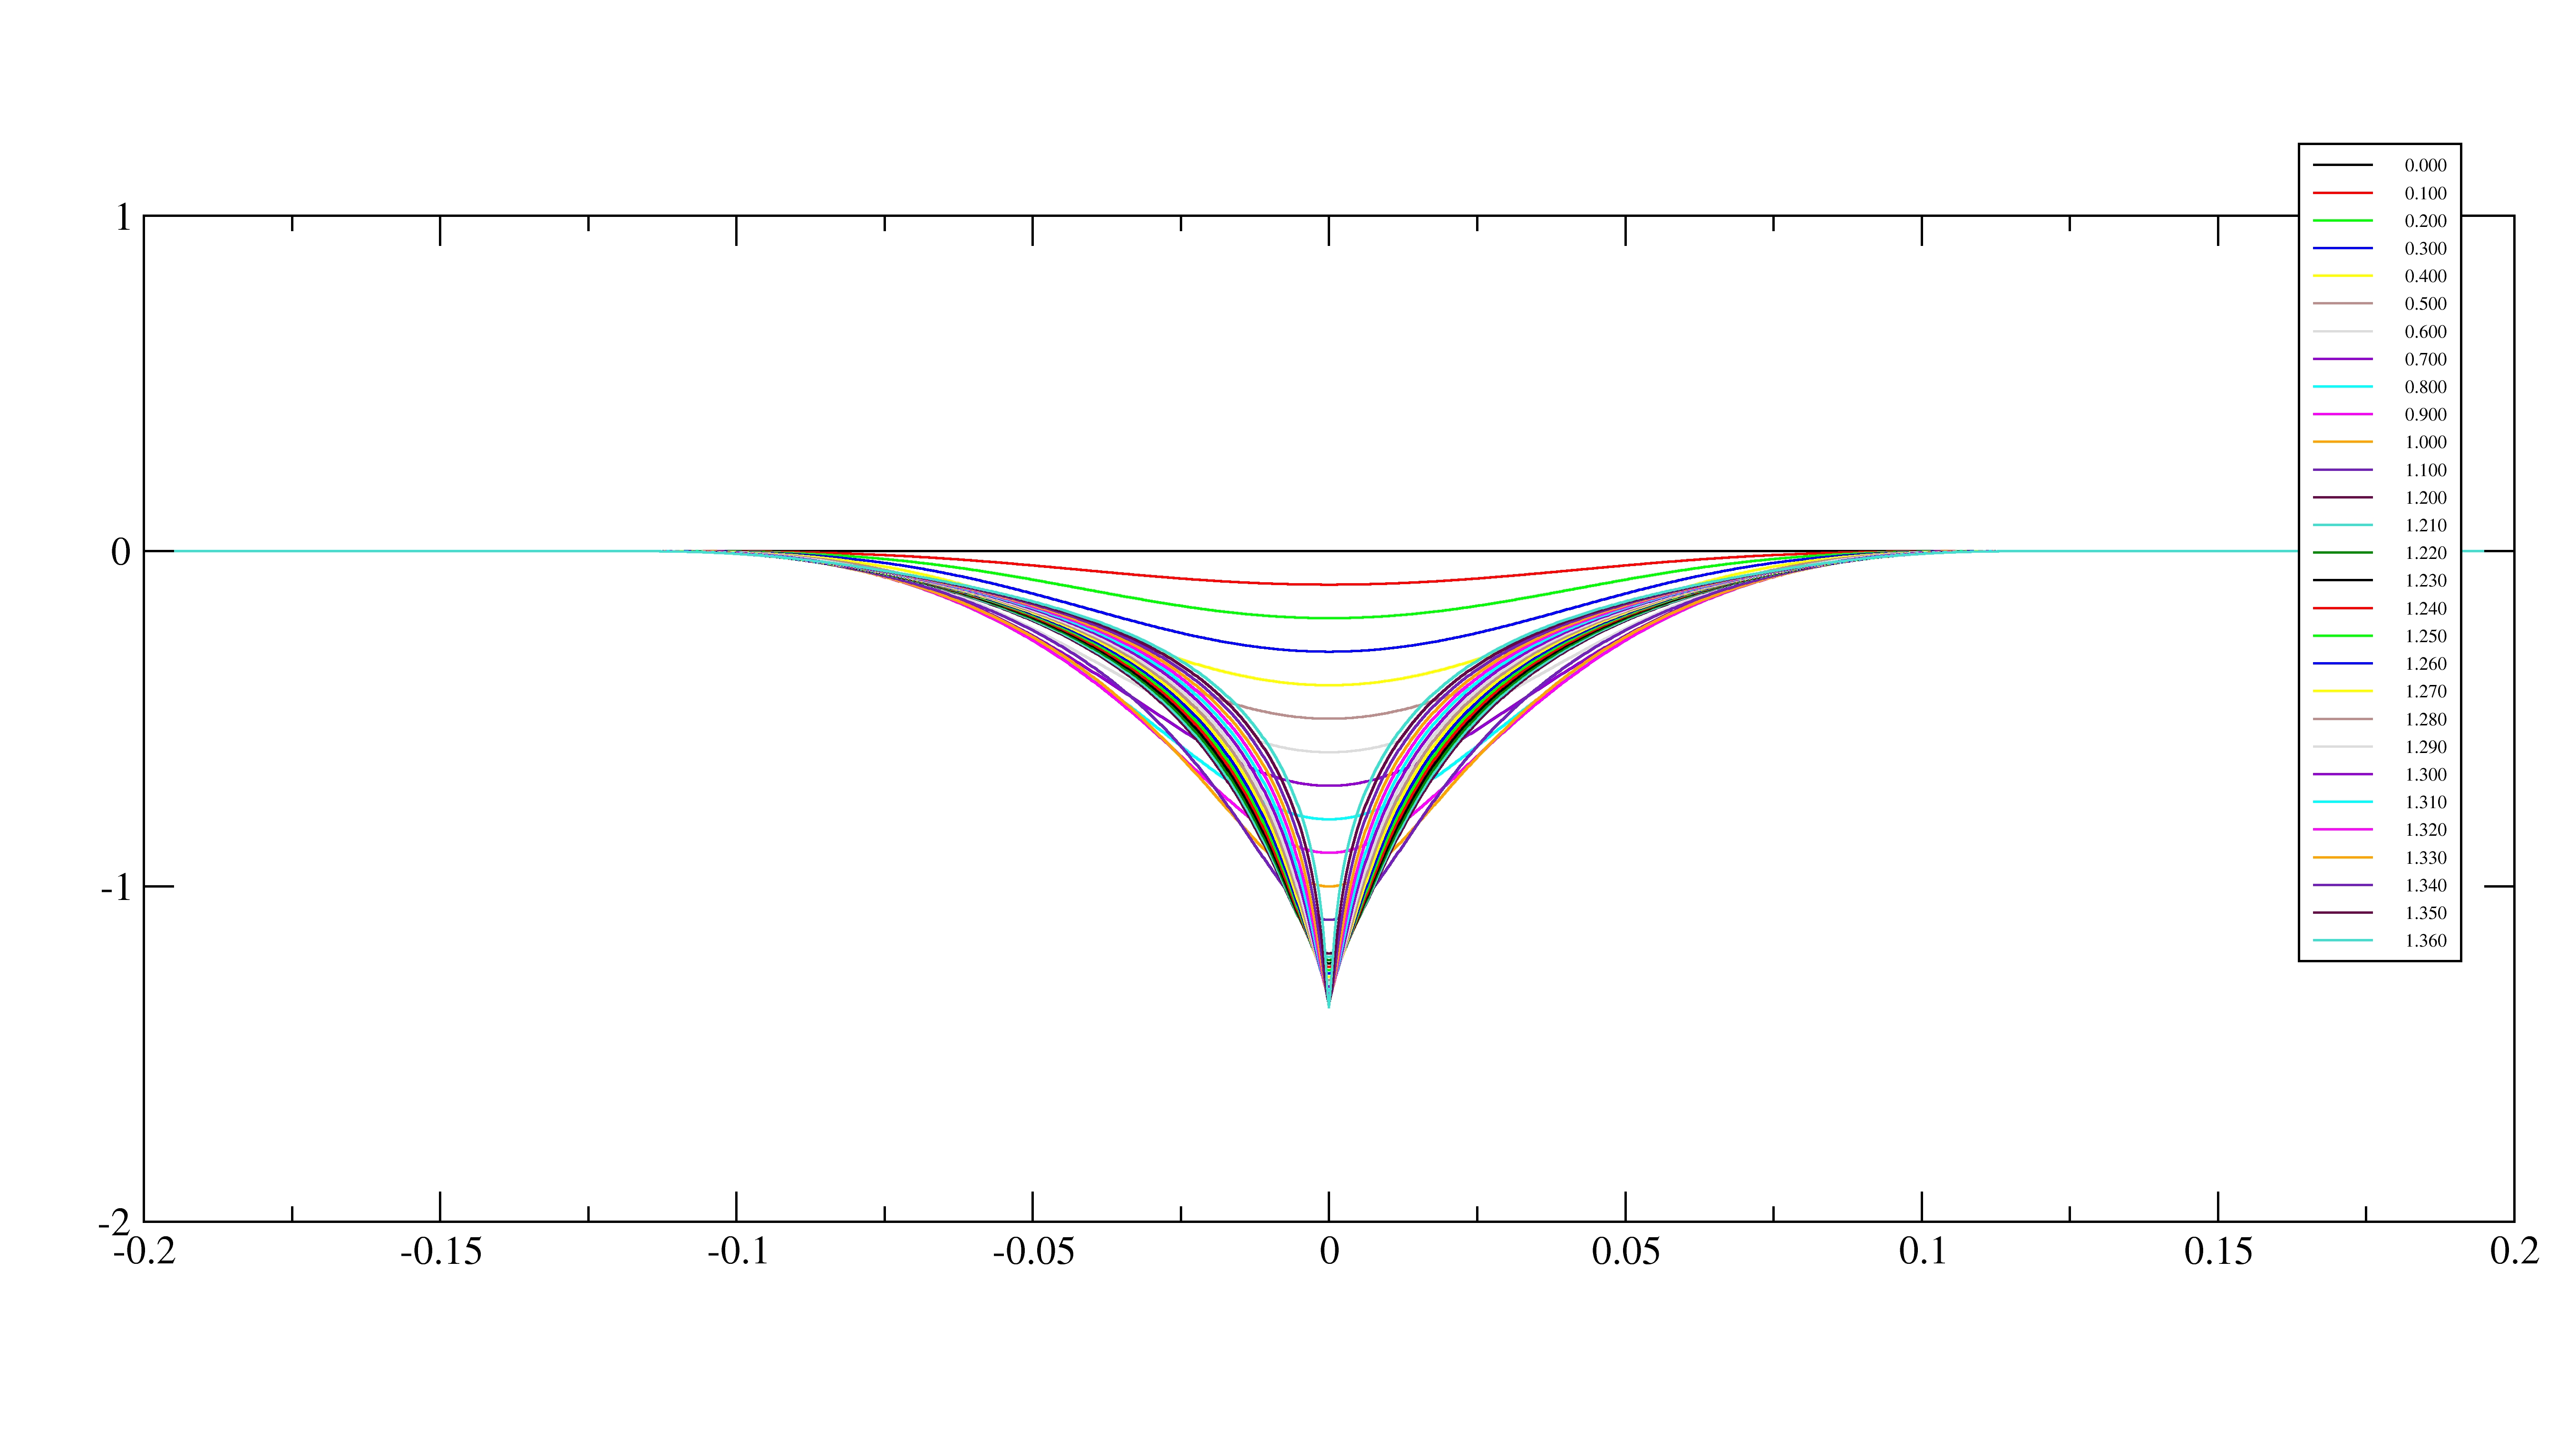
\includegraphics[width=1\textwidth]{uforfig.jpg}
  \caption{{\bf{Local divergence}}: Shown is $u(x,t)$ as a function of
    time, up to divergence.
  }\label{fig:u}
\end{figure}
\begin{figure}[h!]
  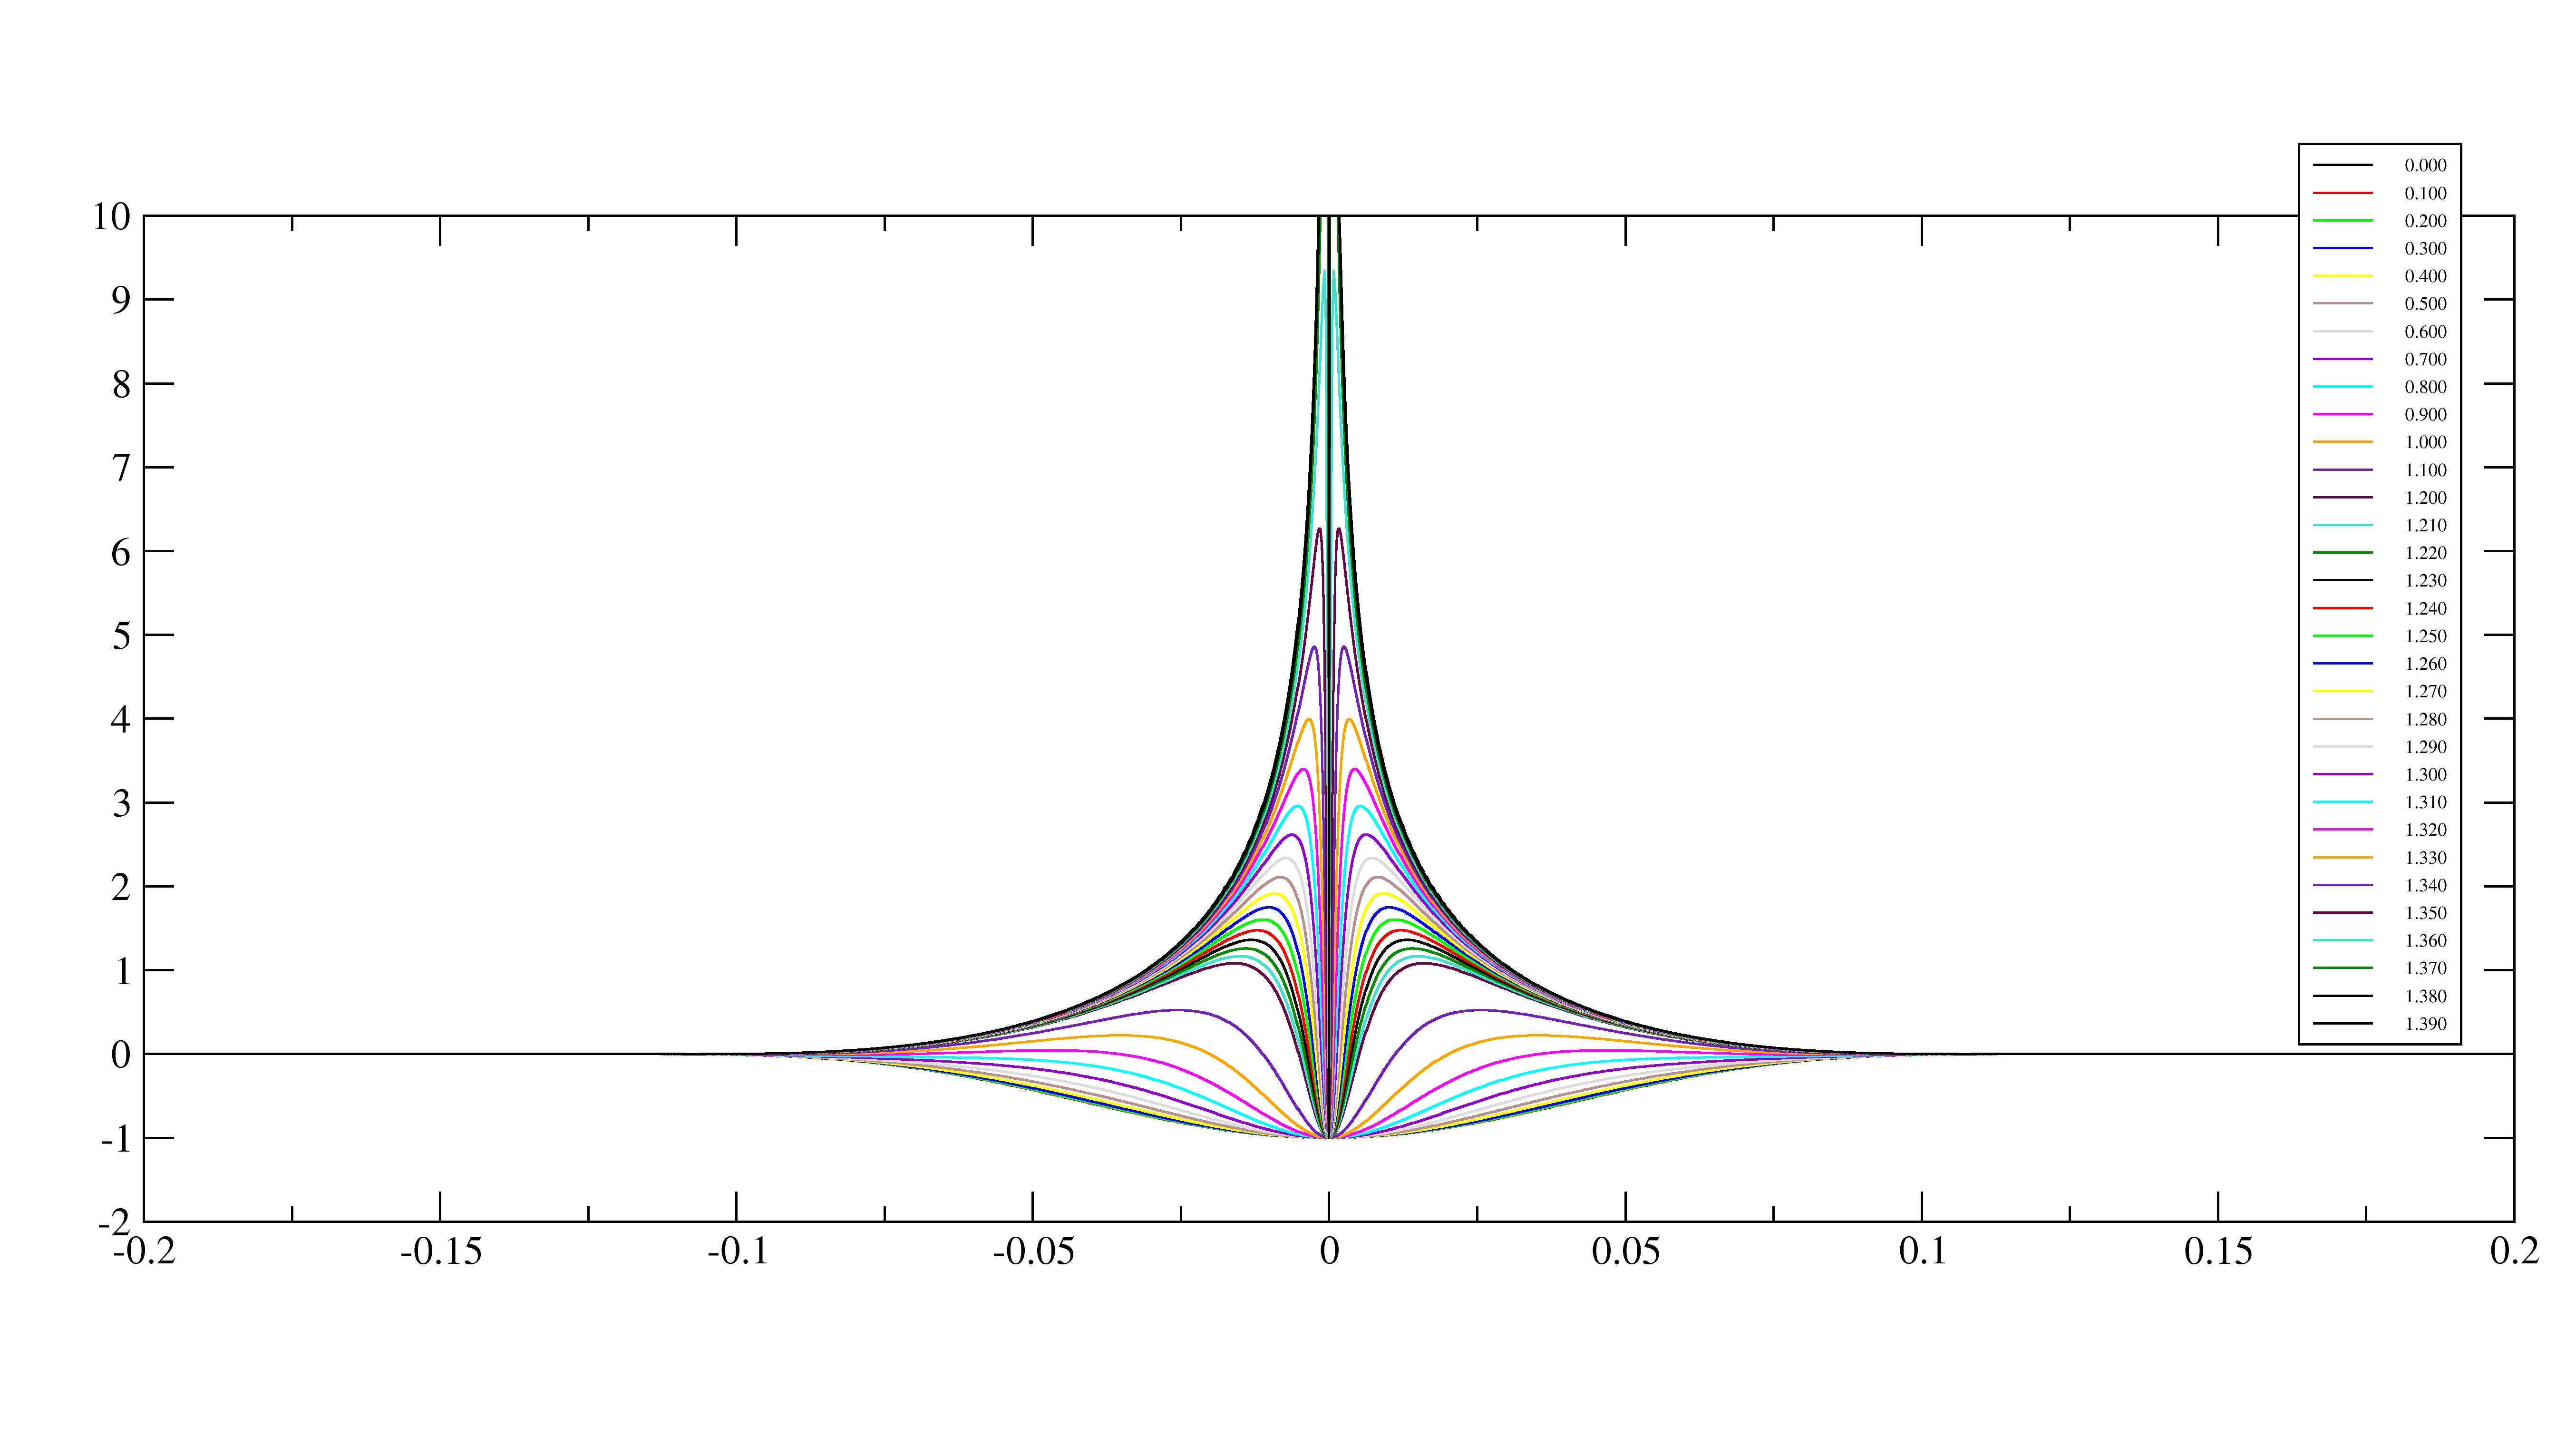
\includegraphics[width=1\textwidth]{utforfig.jpg}
  \caption{{\bf{Local divergence}}: Shown is $u_t(x,t)$ as a function of
    time, up to divergence.
  }\label{fig:ut}
\end{figure}


\newpage


\section{The case $\beta\ne0$}
When $\beta \ne0$ we are interested in the interplay of two types of
divergence, \emph{local} divergence, and \emph{wave divergence}.
In the local divergence, $u$ will diverge near $x=1$ like a special solution of
\eref{eq:main2}. In the wave divergence, there will be a divergence
near the front of the advancing wave.

We illustrate the phenomenology with two numerical simulations,
\fref{fig:peter} and \fref{fig:front}.
\begin{figure}[h!]
  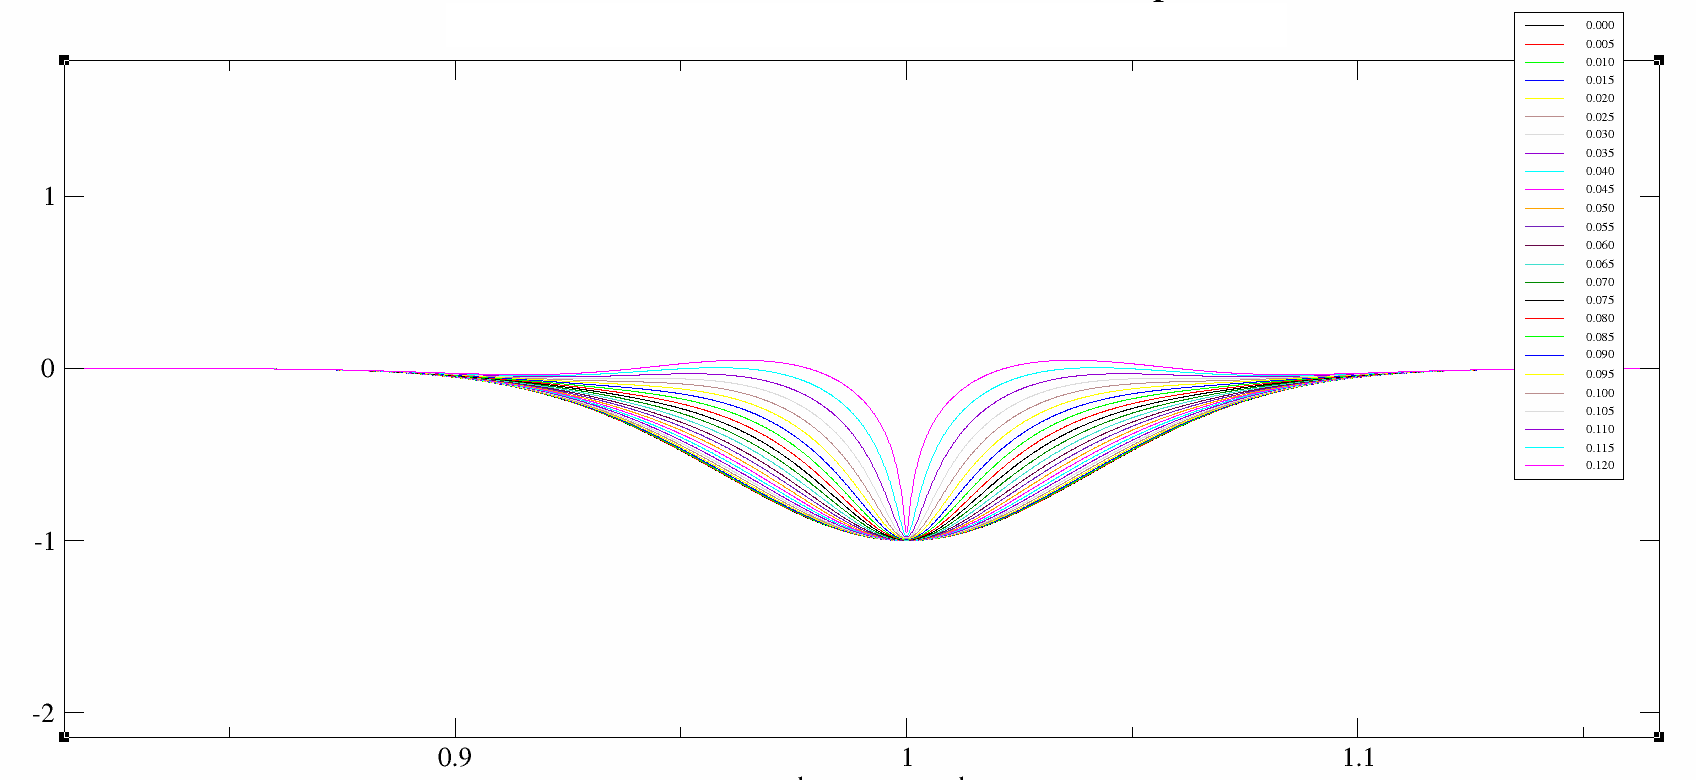
\includegraphics[width=1\textwidth]{peter.png}
  \caption{{\bf{Local divergence}}:The parameters of \eref{eq:main} are $\alpha=5$ and $\beta
    =0.025$ with initial condition
    $u(x,0)=-\exp(-30(x-1)^2)$, $u_t(x,0)=0$. (Numerically we take
    periodic boundary conditions.) Note that the second derivative
    diverges in finite time. The simulation corresponds to $\alpha
    /\beta =200$.
  }\label{fig:peter}
\end{figure}


\begin{figure}[h!]
  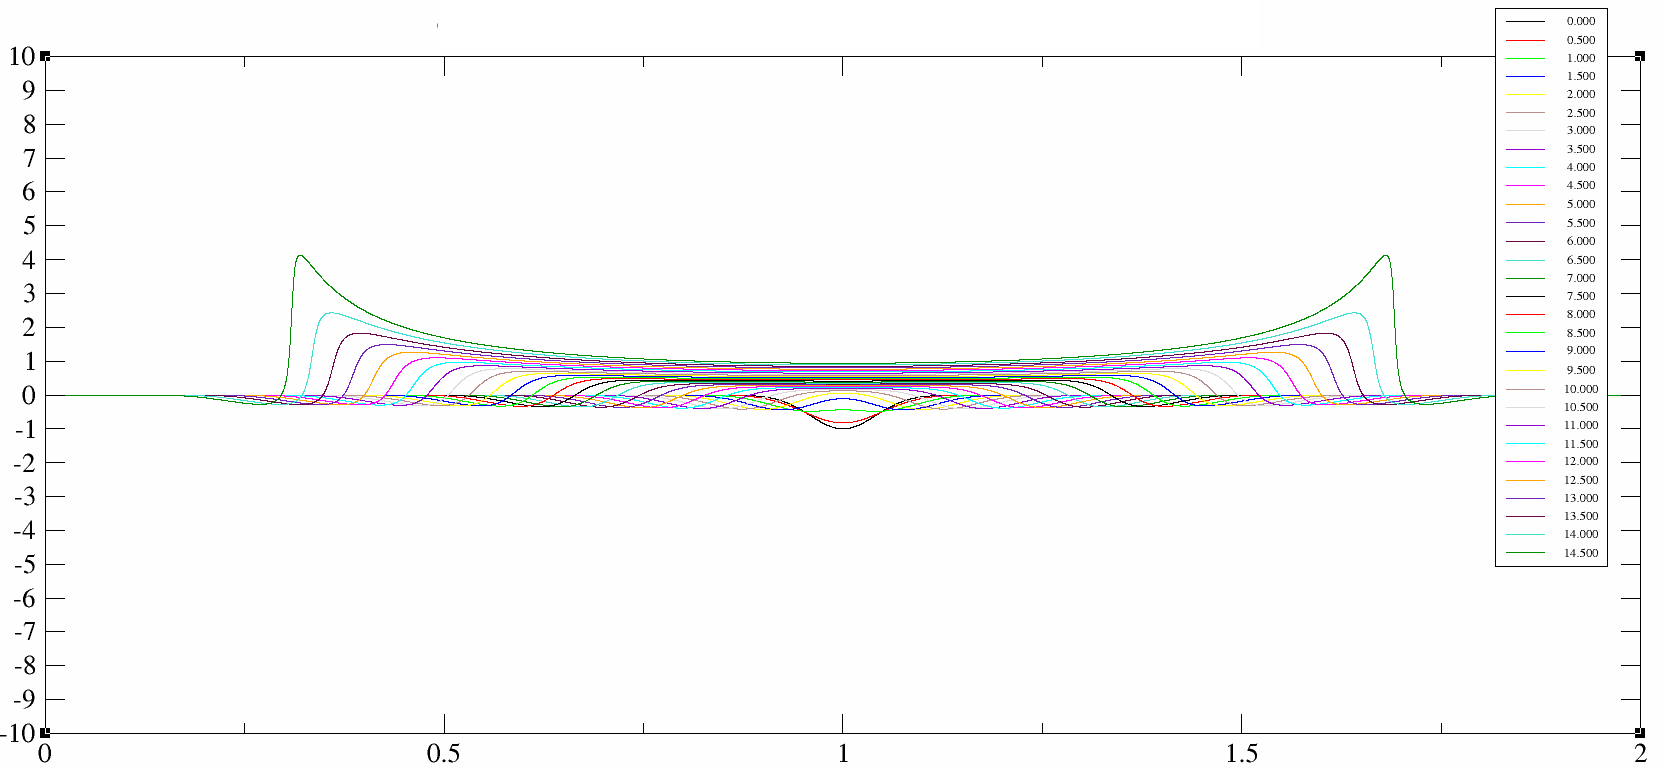
\includegraphics[width=1\textwidth]{divergence.png}
  \caption{{\bf{Wave divergence}}:The nature of divergence ``at infinity.'' As time goes on,
    the support of the function spreads, and the function at the edge
    gets steeper, until the derivative will diverge at some time
    $T_*$.
    The simulation is for the variant equation \eref{eq:main2}, with
    $\alpha=0.01$ and $\beta =0.025$ and initial condition
    $u(x,0)=-\exp(-30(x-1)^2)$, $u_x(x,0)=0$. (Numerically we take
    periodic boundary conditions.) Now, $\alpha /\beta =0.4$
  }\label{fig:front}
\end{figure}

We expect that, for fixed $\alpha /\beta $ a transition between local
divergence and wave divergence will appear, when the initial condition
is fixed. The mathematical situation
for the wave divergence can be explained by an adaptation of the work
of Rammaha \citep{rammaha}. He shows that \eref{eq:main1} will diverge
in finite time under quite weak conditions: We adapt the proof to the
1d case in \tref{thm:t1},  which will be given at the end.

Take as initial conditions smooth
functions $u(x,0)=f(x)$ and $u_t(x,0)=g(x)$, both with compact support
and assume the support is in $|x|<X$. Fix an $X_0<X$ and define
\begin{equa}
  \epsilon = \HALF\int_{x>X_0} (f(x) + (x-X_0) g(x)) \d x~.
\end{equa}
with
\begin{equa}
  M(x)= \HALF \left(f(x) + \int_x^X g(\xi)\d\xi\right)>0
\end{equa}
for all $x\in(X_0,X)$.
We show that the 
solution must diverge before a time
$  T_* $. We do not aim to get the best possible bound on this time.

Rammaha's result can be paraphrased as follows. 
The point of the proofs is that because of the wave character of
\eref{eq:main}, the solution will grow at the advancing front of the
wave. The
qualitative behavior is clearly seen in \fref{fig:front}.

This discussion settles the question of what must happen at the
advancing fronts. However, there can be a local divergence which can
appear earlier in the ``center'' between the waves.

We have considered the shape of the exploding wave front. While we
have no theoretical insights, perhaps the following remarks can help
future research: It seems that the exploding front has a universal
shape, at least near the maximum of the exploding profile.
However, extensive numerical tests show that while these profiles rescale
properly in each instance of the equation, the profiles for
different $\alpha /\beta $ and fixed initial condition seem not to be the same. We tested the ``usual''
rescaling ideas, but they manifestly do not work.






\section{Wave divergence}

  Consider the equation
  \begin{equ}
    u_{tt}-u_{xx}= u_x^2~.
  \end{equ}
  Assume the initial conditions are
  \begin{equa}
    u(x,0)&=f(x)~,\quad
    u_t(x,0)=g(x)~,
  \end{equa}
  with $f$, $g$ having support in $|x|<X$.
  Define, for $x>0$,
  \begin{equ}
    M(x)=\HALF f(x)+\HALF \int_x^X g(\xi)\d\xi~.
  \end{equ}
\begin{theorem}\label{thm:t1}
Assume  there is an $X_0\in (0,X)$ for which $M(x)\ge0$ for all
  $x\in(X_0,X)$,
  and also
  \begin{equ}
    \int_{X_0}^X M(\xi)\d \xi \equiv\epsilon >0~.
  \end{equ}
  Then the local existence time is {\bf{finite}}.
  
 
\end{theorem}
\begin{proof} It suffices to consider the situation where $u(x,0)$ and
  $u_t(x,0)$ have
support in $|x|\le X$, but  we will consider only the side of positive
$x$ in the sequel. Clearly, $u(x,t)=0$ for $x\ge t+X$.
One estimates now the function
\begin{equ}
  H(t)=\int_{X_1}^t (t-\tau )\int _{\tau +X_0}^{\tau +X} u(\xi,\tau
  )\d\xi \,\d\tau ~.
\end{equ}
Here, $X_1=(X-X_0)/2$.
From the definition, we get
\begin{equ}\label{eq:hpp}
  H''(t)=\int _{t +X_0}^{t +X} u(\xi,t)\d\xi~.
\end{equ}
One has the explicit formula
\begin{equ}\label{eq:uxt}
  u(x,t)=u_0(x,t)+\HALF\int_0^t \int_{x-t+\tau }^{x+t-\tau }
  u_x(\xi,\tau )^2 \d\tau \,\d\xi~,
\end{equ}
with the ``free evolution''
\begin{equ}
  u_0(x,t)=\HALF\left(f(x-t)+f(x+t)\right)+\HALF \int_{x-t}^{x+t} g(\xi)\d\xi~.
  \end{equ}
When $x\ge t+X_0$ and $X\ge t \ge X_1$,
then $x+t\ge X$ and therefore $f(x+t)=0$ and therefore, in this region,
\begin{equ}
  u_0(x,t)=\HALF f(x-t) + \HALF\int_{x
    -t}^{x+t} g(\xi) \d \xi~.
\end{equ}
We get from \eref{eq:uxt} and \eref{eq:hpp},
\begin{equ}
  H''(t)=G_0(t)+G_1(t)~,
\end{equ}
with
\begin{equ}
  G_0(t)= \int_{t+X_0}^{t+X}  u_0(x,t)\d x = \int_{t+X_0}^{t+X}
  M(x-t)\d x=\int_{X_0}^X M(x)\d x= \epsilon~,
\end{equ}
by the definition of $\epsilon $ in \tref{thm:t1}.
The nonlinearity leads to
\begin{equ}
  G_1(t)= \int_{t+X_0}^{t+X}\d\xi \int_{0}^{t}\d\tau
  \int_{\xi-t+\tau}^{\xi+t-\tau}\d\eta \,u_x(\eta,\tau)^2~.
\end{equ}
In \lref{lem:3} below, we show
\begin{equa}\label{eq:lem2}
  G_1(t)\ge\frac{1}{t+X_0}\int_{X_1}^t\d\tau  \int_{\tau +X_0}^{\tau +X} \d\xi
  \,(t-\tau )\,(\xi-\tau -X_0) \,u_x(\xi,\tau)^2~.
\end{equa}



We use now the Schwarz inequality in the form
\begin{equ}
  \int \phi \psi = \int \phi^{1/2} (\phi^{1/2}\psi)\le \left(\int
  \phi\psi^2\right)^{1/2} \, (\int \phi)^{1/2}~,
\end{equ}
with $\phi=(t-\tau
)(\xi-\tau -X_0) $ and $\psi=u_x$. This leads to
\begin{equ}
  G_1(t)\ge F^2(t)/J(t)~,
  \end{equ}
with
\begin{equ}
F(t)=\int_{X_1}^t \int_{\tau +X_0}^{\tau +X} (t-\tau
  )(\xi-\tau -X_0) u_x(\xi,\tau )\d \xi \,\d\tau  
\end{equ}
and
\begin{equ}
  J(t)=\int_{X_1}^t \int_{\tau +X_0}^{\tau +X}  (t-\tau
  )(\xi-\tau -X_0)\d\tau \,\d\xi=\frac{(X-X_0)^2(t-X_1)^2}{4}~.
\end{equ}
If we integrate the expression for $F$ by parts (in $\xi$),
we get
\begin{equ}
  F(t)=-\int_{X_1}^t \int_{\tau +X_0}^{\tau +X} (t-\tau
  ) u(\xi,\tau )\d \xi \,\d\tau  = -H(t)~.
\end{equ}
Therefore, we find finally
\begin{equ}\label{eq:final}
  H''(t)\ge G_0(t)+ \frac{H(t)^2}{J(t)}~.
\end{equ}
Fix now $T$ and we will show that the solution cannot exist
for
$T>T_*$, where $T_*$ will be computed in the proof:
We use here Lemma 1 from \citep{rammaha2} adapted to the 1d case.
The ingredients are that
\begin{equ}\label{eq:eps}
  H''(t)\ge G_0(t)=\epsilon >0~,
\end{equ}
for all $t\ge0$ and
\begin{equ}\label{eq:7}
  H''(t)\ge G_1(t)\ge 4\frac{H(t)^2}{(X-X_0)^2 (t-X_1)^2}~,
\end{equ}
for $t>X_1$ (as long as the solution exists). Furthermore, $H(X_1)=H'(X_1)=0$.

Fix now $T_1=2(X_1+1)$. Then, for $t>T_1$, we have $t-X_1>\HALF(t+1)$,
and we replace from now on \eref{eq:7} by the simpler
\begin{equ}\label{eq:Hpp}
  H''(t) \ge K_1 \frac{H(t)^2}{(t+1)^2}~, \text{ for } t>T_1~,
\end{equ}
with $K_1=16/(X-X_0)^2$.



The idea is now to deduce from \eref{eq:eps} and \eref{eq:Hpp} an
inequality of the form
\begin{equ}\label{eq:diverge}
H'(t)\ge C H^{1+\delta}(t)\text{  for  }t>T_*\text{ with
}\delta >0~.
\end{equ}
This implies divergence in finite time,
when $H(T_0)>0$. Indeed, if $H(T_0)=c^{-1/\delta }>0$, then
\begin{equ}\label{eq:diverge2}
  H(t)=\frac{1}{(c-C\delta (t-T_0))^{1/\delta }}~.
\end{equ}
One can reformulate this as follows:
If $H(T_0)=A$ and $A\le 1/e$, the optimizing $\delta $ in
\eref{eq:diverge2} is $\le1$ and therefore
we find that the divergence time is proportional to $-\log(A)$.
Note that, if, for example, the leading edge of the support (at $x=0$) is like
$|x|^2$  for $x<0$, then this will lead to earlier divergence compared
to $|x|^3$.

We now begin the proof proper.
If $B>0$, we will use repeatedly the inequality
\begin{equ}\label{eq:half}
  \frac{x}{x+B}\ge \HALF ~, \text{ for all } x\ge B~.
\end{equ}
From \eref{eq:eps} we find
\begin{equ}\label{eq:181}
  H(t)\ge K_2 \epsilon t^2~, \text{ for all } t>0~,
\end{equ}
with $K_2=\HALF$.

Substituting \eref{eq:181} into \eref{eq:Hpp}, we get
\begin{equ}\label{eq:182}
  H''(t)\ge K_1K_2\epsilon  H(t) \frac{t^2}{(t+1)^2}\ge K_3 \epsilon
  H(t)~, \text { when } t>T_2~,
\end{equ}
for some large enough $T_2=\const T_1$, not depending on $\epsilon $.
Since $H'(t)>0$, we can multiply \eref{eq:182} by $H'$ and write it as
\begin{equ}
 \frac{\d}{\d t}(H'(t)^2)\ge K_3 \epsilon  \frac{\d}{\d t}(H(t)^2) \text { when } t>T_2~.
\end{equ}
We integrate from $T_2$ to $t$ and obtain
\begin{equ}
  H'(t)^2 \ge  K_3\epsilon \left( H(t)^2+H'(T_2)^2-H(T_2)^2\right)=
K_3\epsilon H(t)^2 +K_4\epsilon 
  \text { when } t>T_2~,
\end{equ}
for some $K_4$.
From \eref{eq:eps}, we conclude that for large enough $T_3$, one has
\begin{equ}
K_3\epsilon H(t)^2 +K_4\epsilon \ge K_5\epsilon  H(t)^2~,\text{ when } t>T_3~.
\end{equ}
Combining the last two equations we find
\begin{equ}
  H'(t)\ge K_5^{1/2} \epsilon ^{1/2}  H(t),~
  \text { when } t>T_3~.
\end{equ}
Integrating from $T_3$ to $t$ this leads to
\begin{equ}\label{eq:exp}
  H(t)\ge H(T_3)\exp\left(K_6 \epsilon ^{1/2} (t-T_3)\right)\ge
  H(T_3)\exp\left(\HALF K_6 \epsilon ^{1/2}t\right)~,\text{ when }t>2T_3, 
\end{equ}
with $K_6=K_5^{1/2}$.
Substituting again into \eref{eq:Hpp}, we get
\begin{equ}
  H''(t) \ge K_7 H(t)^{1+\delta } ~,\text{ for any }\delta >0~,
\end{equ}
since the exponential in \eref{eq:exp} (to the power $\delta>0 $) will
dominate the factor $(t+1)^{-2}$ of \eref{eq:Hpp}, if only $t$ is
sufficiently large. (Note that $K_7$ and this new minimal time $T_4$ will
depend on $\delta $.)
We now multiply the last equation by $H'$ and we get
\begin{equ}
  \frac{\d}{\d t}(H'(t)^2) \ge  \frac{2K_7}{2+\delta  }\frac{\d}{\d
    t}\left( H(t)^{2+\delta } \right)~,\text{ for } t>T_4~.
\end{equ}
Integrating from $T_4$ to $t$
we find
\begin{equ}
  H'(t)^2 \ge  \frac{2K_1}{2+\delta  } \left(H(t)^{2+\delta
  }-H(T_{4})^{2+\delta }\right)+H'(T_{4})^2~.
\end{equ}
Taking square roots on both sides and choosing $T_*$
sufficiently larger than $T_4$, we finally arrive at \eref{eq:diverge}
from which we see that there is divergence in finite time, as in \eref{eq:diverge2}.
\end{proof}

We still need to show the inequality \eref{eq:lem2}.
\begin{lemma}\label{lem:3}
  Let
 \begin{equa}
  G_1(t)&= \int_{t+X_0}^{t+X}\d x \int_{0}^{t}\d\tau
  \int_{x-t+\tau}^{x+t-\tau}\d\xi \,u_x(\xi,\tau)^2~.
 \end{equa}
Let $X>X_0>0$, and assume $u_x(x,t)=0$ for all $|x|\ge t+X$, $0\le
t\le T$. Then one has for all $T\ge t\ge X_1=(X-X_0)/2$, the inequality
 \begin{equa}\label{eq:ineq}
  G_1(t)\ge\frac{1}{t+X_0}\int_{X_1}^t\d\tau  \int_{\tau +X_0}^{\tau +X} \d\xi
  \,(t-\tau )\,(\xi-\tau -X_0) \,u_x(\xi,\tau)^2~.
\end{equa}
\end{lemma}
\begin{proof}
\begin{equa}
  G_1(t)&= \int_{t+X_0}^{t+X}\d x \int_{0}^{t}\d\tau
  \int_{x-t+\tau}^{x+t-\tau}\d\xi \,u_x(\xi,\tau)^2\\
&=  \int_{0}^{t}\d\tau\int_{t+X_0}^{t+X}\d x
  \int_{x-t+\tau}^{x+t-\tau}\d\xi \,u_x(\xi,\tau)^2~.\\
\end{equa}
Note that for $t\ge X_1$, the function $u_x(\xi,\tau )$ vanishes for
$\xi\ge\tau +X$. Therefore, since also $2t-\tau \ge \tau $, we find
\begin{equa}
&\int_{0}^{t-X_1}\d\tau\int_{t+X_0}^{t+X}\d x
  \int_{x-t+\tau}^{x+t-\tau}\d\xi \,u_x(\xi,\tau)^2~\\
  =&\int_{0}^{t-X_1}\d\tau
  \int_{\tau +X_0}^{2t+X-\tau }\d \xi
  \int_{t+X_0}^{\xi+t-\tau}\d x \,u_x(\xi,\tau)^2\\
  =&\int_{0}^{t-X_1}\d\tau
  \int_{\tau +X_0}^{\tau +X }\d \xi\,u_x(\xi,\tau)^2
  \int_{t+X_0}^{\xi+t-\tau}1\,\d x~.\\
\end{equa}
Similarly,
\begin{equa}
  &\int_{t-X_1}^t \d \tau \int_{t+X_0}^{t+X}\d x
  \int_{x-t+\tau}^{x+t-\tau}\d\xi \,u_x(\xi,\tau)^2 \\
= &\int_{t-X_1}^{t}\d \tau  \int_{\tau +X_0}^{2t-\tau +X_0}\d\xi
  \,u_x(\xi,\tau)^2\int_{t+X_0}^{\xi+t-\tau } 1 \d
  x\\
  &+\int_{t-X_1}^{t}\d \tau  \int_{2t-\tau +X_0}^{\tau +X}\d\xi
  \,u_x(\xi,\tau)^2\int_{\xi-t+\tau }^{\xi+t-\tau } 1 \d x~.\\
\end{equa}
Therefore, when $t\ge X_1$ the function $G_1$ can be decomposed as
\begin{equa}
  G_1(t)&= \int_0^{t-X_1}\d \tau  \int_{\tau +X_0}^{\tau +X}\d\xi
  \,u_x(\xi,\tau)^2\int_{t+X_0}^{\xi+t-\tau } 1 \d x\\
  &+\int_{t-X_1}^{t}\d \tau  \int_{\tau +X_0}^{2t-\tau +X_0}\d\xi
  \,u_x(\xi,\tau)^2\int_{t+X_0}^{\xi+t-\tau } 1 \d
  x\\
  &+\int_{t-X_1}^{t}\d \tau  \int_{2t-\tau +X_0}^{\tau +X}\d\xi
  \,u_x(\xi,\tau)^2\int_{\xi-t+\tau }^{\xi+t-\tau } 1 \d x~.\\
\end{equa}
The integrals over $\d x$ lead to
\begin{equa}
  G_1(t)&= \int_0^{t-X_1}\d\tau \int_{\tau +X_0}^{\tau +X}\d\xi\,\,(\xi-\tau -X_0) 
  \, u_x(\xi,\tau )^2\\
  &+\int_{t-X_1}^{t}\d \tau\int_{\tau +X_0}^{2t-\tau +X_0}\d\xi\, (\xi-\tau -X_0) 
   \,u_x(\xi,\tau)^2\\
   &+\int_{t-X_1}^{t}\d \tau \,2(t-\tau ) \int_{2t-\tau +X_0}^{\tau +X}\d\xi\,
  \,u_x(\xi,\tau)^2~.\\
\end{equa}
Since
\begin{equa}
  t-\tau \le t+X_0 ~,\text { and\   }\  \xi-\tau -X_0 \le t+X_0~,
\end{equa}
and both are positive,
we find finally that
\begin{equa}
  G_1(t)\ge\frac{1}{t+X_0}\int_{X_1}^t\d\tau  \int_{\tau +X_0}^{\tau +X} \d\xi
  \,(t-\tau )\,(\xi-\tau -X_0) \,u_x(\xi,\tau)^2~.
\end{equa}
\end{proof}

\end{document}



% Biblio:
%@inproceedings{Pich:1998xt,
%    author = "Pich, Antonio",
%    title = "{Effective field theory: Course}",
%    booktitle = "{Les Houches Summer School in Theoretical Physics, Session 68: Probing the Standard Model of Particle Interactions}",
%    eprint = "hep-ph/9806303",
%    archivePrefix = "arXiv",
%    reportNumber = "FTUV-98-46, IFIC-98-47",
%    month = "6",
%    year = "1998"
%}


%@article{HARTMANN2001267,
%title = {Effective Field Theories, Reductionism and Scientific Explanation},
%journal = {Studies in History and Philosophy of Science Part B: Studies in History and Philosophy of Modern Physics},
%volume = {32},
%number = {2},
%pages = {267-304},
%year = {2001},
%note = {Spacetime, Fields and Understanding: Persepectives on Quantum Field},
%issn = {1355-2198},
%doi = {https://doi.org/10.1016/S1355-2198(01)00005-3},
%url = {https://www.sciencedirect.com/science/article/pii/S1355219801000053},
%author = {Stephan Hartmann},
%keywords = {Effective Field Theory, Quantum Field Theory, Renormalisation, Reductionism, Explanation, Pluralism.},
%abstract = {Effective field theories have been a very popular tool in quantum physics for almost two decades. And there are good reasons for this. I will argue that effective field theories share many of the advantages of both fundamental theories and phenomenological models, while avoiding their respective shortcomings. They are, for example, flexible enough to cover a wide range of phenomena, and concrete enough to provide a detailed story of the specific mechanisms at work at a given energy scale. So will all of physics eventually converge on effective field theories? This paper argues that good scientific research can be characterised by a fruitful interaction between fundamental theories, phenomenological models and effective field theories. All of them have their appropriate functions in the research process, and all of them are indispensable. They complement each other and hang together in a coherent way which I shall characterise in some detail. To illustrate all this I will present a case study from nuclear and particle physics. The resulting view about scientific theorising is inherently pluralistic, and has implications for the debates about reductionism and scientific explanation.}
%}

%@article{Cheung:2007st,
%    author = "Cheung, Clifford and Creminelli, Paolo and Fitzpatrick, A. Liam and Kaplan, Jared and Senatore, Leonardo",
%    title = "{The Effective Field Theory of Inflation}",
%    eprint = "0709.0293",
%    archivePrefix = "arXiv",
%    primaryClass = "hep-th",
%    reportNumber = "IC-2007-032",
%    doi = "10.1088/1126-6708/2008/03/014",
%    journal = "JHEP",
%    volume = "03",
%    pages = "014",
%    year = "2008"
%}

%@article{Gubitosi:2012hu,
%    author = "Gubitosi, Giulia and Piazza, Federico and Vernizzi, Filippo",
%    title = "{The Effective Field Theory of Dark Energy}",
%    eprint = "1210.0201",
%    archivePrefix = "arXiv",
%    primaryClass = "hep-th",
%    doi = "10.1088/1475-7516/2013/02/032",
%    journal = "JCAP",
%    volume = "02",
%    pages = "032",
%    year = "2013"
%}


%@article{Weinberg:2008hq,
%    author = "Weinberg, Steven",
%    title = "{Effective Field Theory for Inflation}",
%    eprint = "0804.4291",
%    archivePrefix = "arXiv",
%    primaryClass = "hep-th",
%    reportNumber = "UTTG-01-08",
%    doi = "10.1103/PhysRevD.77.123541",
%    journal = "Phys. Rev. D",
%    volume = "77",
%    pages = "123541",
%    year = "2008"
%}

%@article{SupernovaSearchTeam:1998fmf,
%    author = "Riess, Adam G. and others",
%    collaboration = "Supernova Search Team",
%    title = "{Observational evidence from supernovae for an accelerating universe and a cosmological constant}",
%    eprint = "astro-ph/9805201",
%    archivePrefix = "arXiv",
%    doi = "10.1086/300499",
%    journal = "Astron. J.",
%    volume = "116",
%    pages = "1009--1038",
%    year = "1998"
%}

%@article{Hassani:2019lmy,
%    author = "Hassani, Farbod and Adamek, Julian and Kunz, Martin and Vernizzi, Filippo",
%    title = "{$k$-evolution: a relativistic N-body code for clustering dark energy}",
%    eprint = "1910.01104",
%    archivePrefix = "arXiv",
%    primaryClass = "astro-ph.CO",
%    doi = "10.1088/1475-7516/2019/12/011",
%    journal = "JCAP",
%    volume = "12",
%    pages = "011",
%    year = "2019"
%}
%@article{Hassani:2019wed,
%    author = "Hassani, Farbod and L'Huillier, Benjamin and Shafieloo, Arman and Kunz, Martin and Adamek, Julian",
%    title = "{Parametrising non-linear dark energy perturbations}",
%    eprint = "1910.01105",
%    archivePrefix = "arXiv",
%    primaryClass = "astro-ph.CO",
%    doi = "10.1088/1475-7516/2020/04/039",
%    journal = "JCAP",
%    volume = "04",
%    pages = "039",
%    year = "2020"
%}


%@article{Adamek:2016zes,
%    author = "Adamek, Julian and Daverio, David and Durrer, Ruth and Kunz, Martin",
%    title = "{gevolution: a cosmological N-body code based on General Relativity}",
%    eprint = "1604.06065",
%    archivePrefix = "arXiv",
%    primaryClass = "astro-ph.CO",
%    doi = "10.1088/1475-7516/2016/07/053",
%    journal = "JCAP",
%    volume = "07",
%    pages = "053",
%    year = "2016"
%}
